\chapter{Work Experience} % Main chapter title

\label{Chapter2} % Change X to a consecutive number; for referencing this chapter elsewhere, use \ref{Chapter2}

\lhead{Chapter 2. \emph{Work Experience}} % Change X to a consecutive number; this is for the header on each page - perhaps a shortened title

I have had a total of six work placements since the start of my gap year.
Figure \ref{timeline} provides a timeline of the companies I have worked at.
The focus of this chapter will be on my placement at Sunamp, which was specifically done as part of my \textit{Industrial Project}.
After describing my experience at Sunamp, I will briefly describe my other work experiences.

\begin{figure}[htbp]
	\centering
	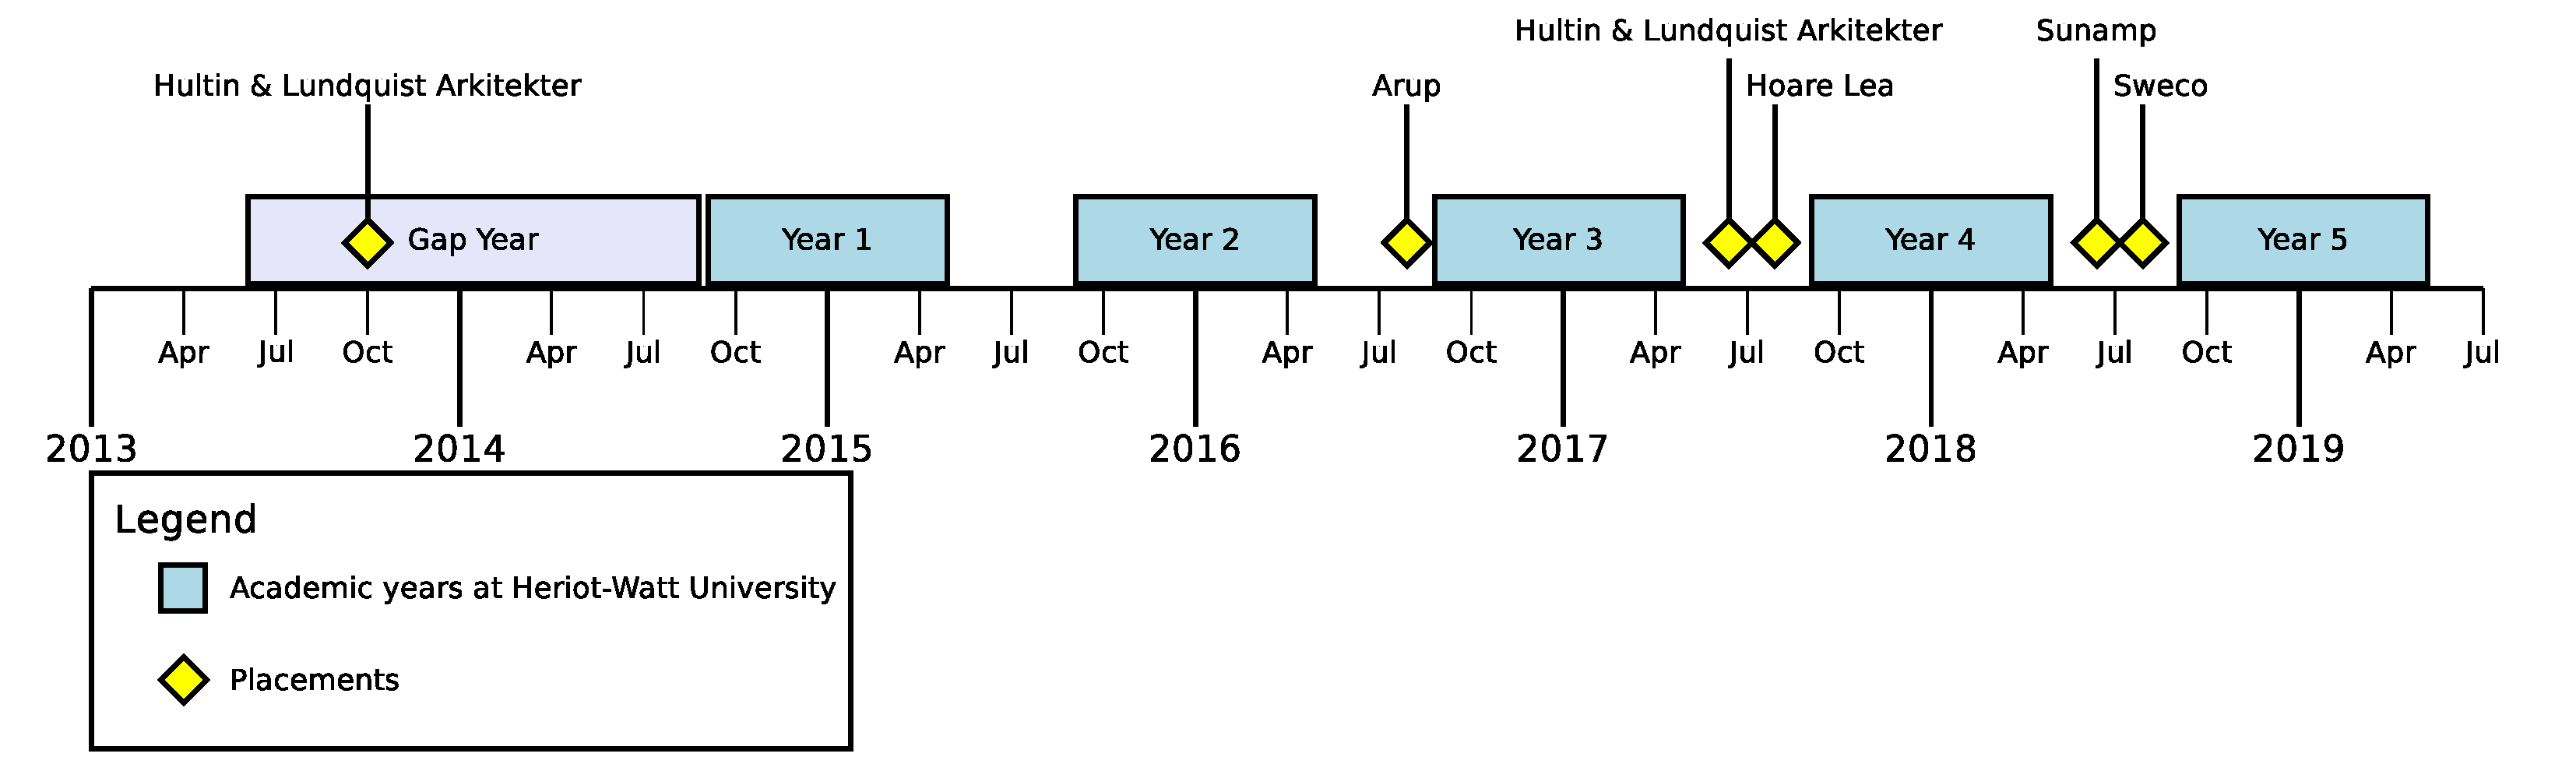
\includegraphics[width=\textwidth]{figures/IP-Timeline.eps}
	\rule{\textwidth}{0.5pt} % use line???
	\caption{Timeline of my work placements since my pre-university gap year.}
	\label{timeline}
\end{figure}


%----------------------------------------------------------------------------------------
%	SECTION 1
%----------------------------------------------------------------------------------------

\section{Sunamp, July - August 2018}

Sunamp is a newly established business that specialises in the research, production and sales of heat batteries that are based on phase change materials (PCMs).
The PCMs, developed and manufactured by Sunamp, are non-toxic, non-flammable, eco-friendly and patented in the UK and China, with patents pending in other countries \citep{SunampAutomotive}.
The PCMs operate at different temperatures, allowing the storage of heat (up to 1000$^{\circ}$C) or coolth (less than 0$^{\circ}$C) (see Figure \ref{pcm_temp_range}).
Currently, the company's main markets are buildings, where their heat batteries can be used for the production of hot water and space heating, and automobiles, where their heat batteries can be used for the refrigeration of transported goods.

\begin{figure}[htbp]
	\centering
	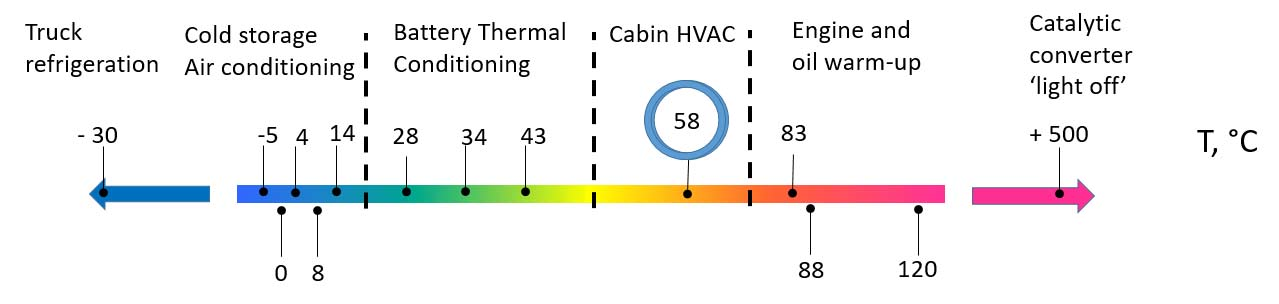
\includegraphics[width=\textwidth]{figures/temperature-range-of-PCMs.jpg}
	\rule{\textwidth}{0.5pt} % use line???
	\caption{The temperature range of Sunamp's PCMs in degrees Celsius \citep{SunampAutomotive}.}
	\label{pcm_temp_range}
\end{figure}

Sunamp was founded by Andrew Bissell (CEO) and is based in Macmerry, East Lothian.
They have a small office building, which features a workshop and chemistry laboratory on the ground floor and an open-plan office on the first floor, and a factory across the road where they have additional test facilities but primarily do large-scale manufacturing and packaging of heat batteries.
Around 20 people work in the office and five in the factory.


%-----------------------------------
%	SUBSECTION 1
%-----------------------------------

\subsection{Description of work experience}

My placement at Sunamp started on Tuesday 3\textsuperscript{rd} July 2018 and ended on Friday 10\textsuperscript{th} August 2018.
I worked a total of 198 hours there across six weeks, averaging at about 6.8 hours of work per day (see log in Appendix ... \hl{blur out sensitive info before adding to appendix}).
\hl{My purpose/ job description ...}
My time at Sunamp can roughly be divided up into two \hl{areas/ aspects}: learning about Sunamp's work and development, and producing work for Sunamp.


\subsubsection{Learning about Sunamp}

The majority of my first week at Sunamp consisted of my familiarisation with the company and their products.
The week started with an induction from Susan Lang-Bissell (MD) where we went over my contract, office information, health and safety regulations (amongst other things) and I got a brief tour of the factory.
The induction was followed by an introduction from Joan Pisanek, the Business Development Manager, to UniQ (Sunamp's latest range of heat batteries for buildings) and some of Sunamp's projects.
I used the rest of the week to familiarise myself with and try to understand their products by consulting Joan's PowerPoint presentations and the UniQ manuals, working through Joan's Buchlyvie project (\hl{see Appendix ...}), and attempting a UniQ Product Training Exercise developed by Sandy.

Santokh Gataora, \hl{colloquially known as} Sandy, is Sunamp's Technical Director.
He has a vast experience in building services engineering and helped develop the UniQ product range.
He writes and continues to refine the UniQ manuals as he guides the company in the engineering and application aspects of their UniQ heat batteries in buildings.
When I joined the company, UniQ was a very recent development that the sales team was still learning about.
The week I arrived at Sunamp, Sandy had sent out an exercise for the sales team to complete for the following week's UniQ Product Training Workshop.
The exercise instructions and my answer \hl{can be found in Appendix ... blur out people's names in email}.
I went on to attend the training workshop, where the sales team and I learned about the UniQ product range in greater depth and briefly went over the solution to the exercise.
\hl{Comment on my answer vs. solution?}

During my second and third weeks at Sunamp, I received more thorough tours of the factory, workshop and chemistry laboratory.
At the factory I got an understanding of the assembly of the heat batteries.
This broadly consists of the selection of a heat exchanger, the installation of the heat exchanger and pipes inside an insulated container, the sealing of the container, the mixing tank for the PCM, the pouring of the PCM into the container, and the cooling-off of the finalised heat battery for the next few days.
\hl{Sketch cross-section of heat battery! Am I allowed though?}

During the workshop and laboratory tour, I gained a deeper understanding of the making and performance of the PCMs and the selection of materials that go inside a heat battery.
Some of the things I learned are:
\begin{itemize}
    \item The high energy density of the PCMs is what allows Sunamp's heat batteries to be 2-4 times smaller than their equivalent hot water cylinders.
    \item Sunamp's chemists cycle and analyse PCM mixtures through solid-liquid and liquid-solid phase transitions to assess the stability of the mixtures' phase transitions over time. The more stable the transitions are, the more suitable they are to be used in heat batteries.
    \item The chemists also need to test their supplier's materials for impurities which can significantly degrade the performance of PCM mixtures.
    \item Different PCM mixtures can react differently to aluminium and copper, the main metals that heat exchangers are built from. Sunamp typically uses all-aluminium finned-tube heat exchangers, but they'll sometimes create a PCM which corrodes aluminium. In these cases they might need to consider using copper-based heat exchangers, which are more expensive but might work out cheaper in the long-run when compared to the capital and operational costs of the heat batteries' equivalent hot water cylinders.
    \item Working with cold, medium and high temperature ranges, the chemists need to ensure that the plastic material of the container which holds the PCM can tolerate that PCM's temperature range. Therefore Sunamp typically uses different materials for containers that carry cold and warm/ hot PCMs.
\end{itemize}

During my fourth and fifth weeks at Sunamp, I attended to two presentations.
The first was a summary of the research carried out by two chemistry students that had spent the past year working on their dissertations at Sunamp.
I gained some insight into the technical aspects of the development of PCMs and was impressed that one of the student's PCMs might soon become patented and used for refrigeration in vehicles.
Sandy gave the second presentation which was an overview of the new UniQ product range to the whole company.
I think this was especially insightful for the chemists and engineers who are specialised in their specific areas and might not always see how all of their work contributes to the end-product (heat batteries) and their application (heating space and water in buildings).

During my sixth (and final) week, I was part of the tour and planning of Sunamp's Experience Room.
This room is designed to look and feel like a home, with a kitchen-like decor and sink in one corner.
One of the purposes of this room, which was still under construction, is to showcase Sunamp's heat batteries to customers by comparing them to their large equivalents on the common marketplace (e.g. hot water cylinders) and by showing how they integrate into a building and its systems (e.g. heat pumps
and boilers).
The second purpose of this room is for workshops where one is trained how to install Sunamp's heat batteries.

Throughout my brief placement at Sunamp, there has been a sense of rapid development and expansion.
The company started out by manufacturing batteries inside a small workshop, which has now grown into a factory which is still evolving with the construction of new testing facilities and training/ marketing spaces.
The company continues to recruit more engineers and scientists.
It also seems like more customers are hearing about and taking interest in Sunamp's heat batteries, in the UK and abroad.

\hl{See notebook notes on how to demonstrate technical understanding.}



\subsubsection{Producing work for Sunamp}

% Ohhhh come on! I gotta write! Just blow off some steam. It doesn't have to be all thought out and structured to begin with. Just keep the hand on the keyboard and type! As Moira says, "Be confident." :D

I joined Sunamp in the wake of the development of their new product range called UniQ.
UniQ had been developed by Sunamp's engineers, notably Sandy, and explained in a manual.
However, the manual was too large and technical for the sales team (headed by Joan) to understand, navigate and use to efficiently match customers with the most suitable UniQ products.
Therefore, my purpose at Sunamp was to bridge the gap between engineering and sales.
This was to be done by creating concise and user-friendly documentation that would introduce and explain the UniQ range to customers and even be used by the sales team as an aide-memoire.
This project mainly consisted of me presenting existing content in new ways and boiling down a lot of technical \hl{information/ features} to meaningful and useful information and benefits for customers.

I started working on my project during my second week at Sunamp and completed it on my last day.
From my log, I have deducted that I worked \hl{at least/ more than} 138 hours on this project, which accounts for 70\% of my time at Sunamp.
This includes the time I spent working autonomously, meetings, \hl{investigations}, and my final presentation.

\hl{use hidden slide to give overview of work produced then dive into headings to discuss each separately.}



%-----------------------------------
%	SUBSECTION 2
%-----------------------------------

\subsection{Analysis of/ Reflection on work experience}


%%%%%%%%%%%%%%%%%%%%%%%%%%%%%%%%%%%%%%%%%%%%%%%%%
\begin{comment}

\subsection{Application Process}

I learned about the opportunity of two paid placements with immediate start at Sunamp through David Campbell, the D11PJ course leader.
He had asked applicants for this placement to send him 100 words broadly describing their strengths and preferences, which he would then forward to Sunamp.
Hamish, a coursemate of mine, and I were both interested in this opportunity.
\hl{My hundred-word application went as follows:}

Strengths:
\begin{itemize}
	\item I am very familiar with the BIM process, having written a dissertation on collaboration with regards to BIM.
	\item I have work experience in mechanical and electrical consulting engineering.
	\item Organised, flexible, independent and cooperative.
\end{itemize}
Skills:
\begin{itemize}
	\item Advanced skills in Microsoft Office packages and Bluebeam Revu.
	\item Intermediate skills in LaTeX.
	\item Basic modelling skills in Revit, AutoCAD and IES-VE.
	\item Fluent in three languages (English, Swedish and French) with basic knowledge of Spanish.
\end{itemize}
Preferences/ interests:
\begin{itemize}
	\item Highly interested in learning about your application of Phase Change Materials in thermal storage batteries.
	\item Also interested in working with BIM and learning Bentley’s Hevacomp software packages.
\end{itemize}

After the applications, David introduced the two of us to Susan Lang-Bissell, the Managing Director (MD) of Sunamp, via email.
David asked us to liaise with Susan to arrange a meeting.
To do this, Hamish and I first established our availabilities in the upcoming days.
I then volunteered to liaise with Susan via email on our behalf to find a suitable date and time.

\hl{Try to be more reflective, and less descriptive.
Maybe record (vocally) the story, and then reflect on it out loud. THEN write about it.}

\end{comment}
